\documentclass{assignment}
\ProjectInfos{量子信息导论}{PHYS5251P}{2021-2022 学年第一学期}{第一次作业}{截止日期:2021. 10. 13(周三)}{陈稼霖}[https://github.com/Chen-Jialin]{SA21038052}

\begin{document}
\begin{prob}
    计算二元对称信道的信道容量.
\end{prob}
\begin{sol}
    对二元对称信道, 设信源发送信号为 $X\in\{0,1\}$, 经信道传输后信宿接收信号为 $Y\in\{0,1\}$, 信道如图 \ref{1-info channel} 所示:

    \begin{figure}[H]
        \centering
        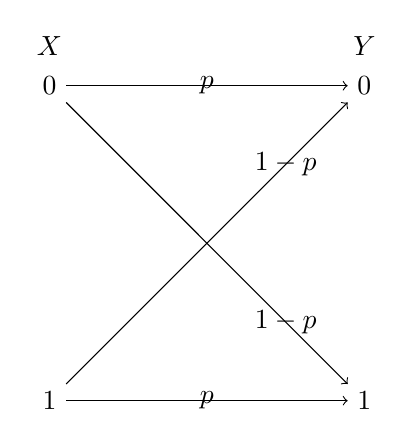
\begin{tikzpicture}
            \node at(0,4.5){$X$};
            \node at(4,4.5){$Y$};
            \node(1)at(0,4){$0$};
            \node(2)at(0,0){$1$};
            \node(3)at(4,4){$0$};
            \node(4)at(4,0){$1$};
            \node at(2,0){$p$};
            \node at(2,4){$p$};
            \node at(3,1){$1-p$};
            \node at(3,3){$1-p$};
            \draw[->](1)--(3);
            \draw[->](1)--(4);
            \draw[->](2)--(3);
            \draw[->](2)--(4);
        \end{tikzpicture}
        \caption{二元对称信道}
        \label{1-info channel}
    \end{figure}

    即
    \begin{align}
        P(Y=0\mid X=0)=&P(Y=1\mid X=1)=p,\\
        P(Y=1\mid X=0)=&P(Y=0\mid X=1)=1-p.
    \end{align}
    $X$ 与 $Y$ 的互信息量为
    \begin{align}
        I(X;Y)=H(Y)-H(Y\mid X),
    \end{align}
    其中 $Y$ 的信息熵为
    \begin{align}
        \notag H(Y)=&-P(Y=0)\log_2P(Y=0)-P(Y=1)\log_2P(Y=1)\\
        \notag=&-P(Y=0)\log_2P(Y=0)-[1-P(Y=0)]\log_2[1-P(Y=0)]\\
        \leq&-\frac{1}{2}\log_2\frac{1}{2}-\frac{1}{2}\log_2\frac{1}{2}=1,
    \end{align}
    而 $Y\mid X$ 的条件熵
    \begin{align}
        \notag H(Y\mid X)=&-P(X=0)[P(Y=0\mid X=0)\log_2P(Y=0\mid X=0)+P(Y=1\mid X=0)\log_2P(Y=1\mid X=0)]\\
        \notag&-P(X=1)[P(Y=0\mid X=1)\log_2P(Y=0\mid X=1)+P(Y=1\mid X=1)\log_2P(Y=1\mid X=1)]\\
        \notag=&-P(X=0)[p\log_2p+(1-p)\log_2(1-p)]-P(X=1)[(1-p)\log_2(1-p)+p\log_2p]\\
        =&-p\log_2p-(1-p)\log_2(1-p).
    \end{align}
    故二元对称信道的信道容量为
    \begin{align}
        C=\max_{P(X=0)}I(X;Y)=1+p\log_2p+(1-p)\log_2(1-p).
    \end{align}
\end{sol}

\begin{prob}
    空间 $H$ 中存在两组正交归一化态 $\{\lvert\psi_i\rangle\}$、$\{\lvert\tilde{\psi}_i\rangle\}$, 则存在幺正变换 $U$, 使得 $U\lvert\psi_i\rangle=\lvert\tilde{\psi}_i\rangle$, 试构造该 $U$ 变换.
\end{prob}
\begin{sol}
    构造
    \begin{align}
        U=\sum_i\lvert\tilde{\psi}_i\rangle\langle\psi_i\rvert,
    \end{align}
    则 $U$ 满足变换
    \begin{align}
        U\lvert\psi_i\rangle=\sum_j\lvert\tilde{\psi}_j\rangle\langle\psi_j\vert\psi_i\rangle=\sum_j\delta_{ij}\lvert\tilde{\psi}_j\rangle=\lvert\tilde{\psi}_i\rangle,\quad\forall i,
    \end{align}
    且 $U$ 是幺正的:
    \begin{align}
        U^{\dagger}U=UU^{\dagger}=\left(\sum_i\lvert\psi_i\rangle\langle\tilde{\psi}_i\rvert\right)\left(\sum_j\lvert\tilde{\psi}_j\rangle\langle\psi_j\rvert\right)=\sum_{ij}\delta_{ij}\lvert\psi_i\rangle\langle\psi_j\rvert=\sum_i\lvert\psi_i\rangle\langle\psi_i\rvert=I.
    \end{align}
\end{sol}

\begin{prob}
    空间 $H$ 中存在两组归一化态 $\{\lvert\psi_i\rangle\}$、$\{\lvert\tilde{\psi}_i\rangle\}$, 它们满足: $\forall i,j$, 有 $\langle\psi_i\vert\psi_j\rangle=\langle\tilde{\psi}_i\vert\tilde{\psi}_j\rangle$. 请证明, 则存在 $U$, 使得 $U\lvert\psi_i\rangle=\lvert\tilde{\psi}_i\rangle$, 并构造出该 $U$ 变换.
\end{prob}
\begin{sol}
    设
    \begin{align}
        U=\sum_{jk}a_{jk}\lvert\tilde{\psi}_j\rangle\langle\psi_k\rvert.
    \end{align}
    要使 $U\lvert\psi_i\rangle=\lvert\tilde{\psi}_i\rangle$, 即需
    \begin{gather}
        U\lvert\psi_i\rangle=\sum_{jk}a_{jk}\lvert\tilde{\psi}_j\rangle\langle\psi_k\vert\psi_i\rangle=\sum_j\left(\sum_ka_{jk}\langle\psi_k\vert\psi_i\rangle\right)\lvert\tilde{\psi}_j\rangle=\lvert\tilde{\psi}_i\rangle,\quad\forall i,\\
        \Longrightarrow\sum_ka_{jk}\langle\psi_k\vert\psi_i\rangle=\delta_{ij},\quad\forall i,j,\\
        \Longrightarrow AB=I
    \end{gather}
    其中矩阵
    \begin{align}
        A=&\begin{bmatrix}
            a_{11}&a_{12}&\cdots&a_{1n}\\
            a_{21}&a_{22}&\cdots&a_{2n}\\
            \vdots&\vdots&\ddots&\vdots\\
            a_{n1}&a_{n2}&\cdots&a_{nn}
        \end{bmatrix},\\
        B=&\begin{bmatrix}
            \langle\psi_1\vert\psi_1\rangle&\langle\psi_1\vert\psi_2\rangle&\cdots&\langle\psi_1\vert\psi_n\rangle\\
            \langle\psi_2\vert\psi_1\rangle&\langle\psi_2\vert\psi_2\rangle&\cdots&\langle\psi_2\vert\psi_n\rangle\\
            \vdots&\vdots&\ddots&\vdots\\
            \langle\psi_n\vert\psi_1\rangle&\langle\psi_n\vert\psi_2\rangle&\cdots&\langle\psi_n\vert\psi_n\rangle
        \end{bmatrix}.
    \end{align}

    因此我们只需由上式构造矩阵 $B$, 再计算
    \begin{align}
        A=B^{-1},
    \end{align}
    然后构造
    \begin{align}
        U=\sum_{jk}a_{jk}\lvert\tilde{\psi}_j\rangle\langle\psi_k\rvert
    \end{align}
    即可满足 $U\lvert\psi_i\rangle=\lvert\tilde{\psi}_i\rangle$.
\end{sol}

\begin{prob}
    对两比特态 $\lvert\phi\rangle=\frac{1}{\sqrt{2}}\lvert 0\rangle_A\left(\frac{1}{2}\lvert 0\rangle_B+\frac{\sqrt{3}}{2}\lvert 1\rangle_B\right)+\frac{1}{\sqrt{2}}\lvert 1\rangle_A\left(\frac{\sqrt{3}}{2}\lvert 0\rangle_B+\frac{1}{2}\lvert 1\rangle_B\right)$,
    \begin{itemize}
        \item[i)] 求约化密度矩阵 $\rho_A$, $\rho_B$;
        \item[ii)] 求 $\lvert\phi\rangle$ 的 Schmidt 分解形式.
    \end{itemize}
\end{prob}
\begin{sol}
    \begin{itemize}
        \item[1)] 复合系统的密度矩阵为
        {\scriptsize
        \begin{align}
            \notag\rho_{AB}=&\lvert\phi\rangle\langle\phi\rvert\\
            \notag=&\left[\frac{1}{\sqrt{2}}\lvert 0\rangle_A\left(\frac{1}{2}\lvert 0\rangle_B+\frac{\sqrt{3}}{2}\lvert 1\rangle_B\right)+\frac{1}{\sqrt{2}}\lvert 1\rangle_A\left(\frac{\sqrt{3}}{2}\lvert 0\rangle_B+\frac{1}{2}\lvert 1\rangle_B\right)\right]\left[\frac{1}{\sqrt{2}}\langle 0\rvert_A\left(\frac{1}{2}\langle 0\rvert_B+\frac{\sqrt{3}}{2}\langle 1\rvert_B\right)+\frac{1}{\sqrt{2}}\langle 1\rvert_A\left(\frac{\sqrt{3}}{2}\langle 0\rvert_B+\frac{1}{2}\langle 1\rvert_B\right)\right]\\
            \notag=&\frac{1}{8}\lvert 0\rangle_A\lvert 0\rangle_B\langle 0\rvert_A\langle 0\rvert_B+\frac{\sqrt{3}}{8}\lvert 0\rangle_A\lvert 0\rangle_B\langle 0\rvert_A\langle 1\rvert_B+\frac{\sqrt{3}}{8}\lvert 0\rangle_A\lvert 0\rangle_B\langle 1\rvert_A\langle 0\rvert_B+\frac{1}{8}\lvert 0\rangle_A\lvert 0\rangle_B\langle 1\rvert_A\langle 1\rvert_B\\
            \notag+&\frac{\sqrt{3}}{8}\lvert 0\rangle_A\lvert 1\rangle_B\langle 0\rvert_A\langle 0\rvert_B+\frac{3}{8}\lvert 0\rangle_A\lvert 1\rangle_B\langle 0\rvert_A\langle 1\rvert_B+\frac{3}{8}\lvert 0\rangle_A\lvert 1\rangle_B\langle 1\rvert_A\langle 0\rvert_B+\frac{\sqrt{3}}{8}\lvert 0\rangle_A\lvert 1\rangle_B\langle 1\rvert_A\langle 1\rvert_B\\
            \notag+&\frac{\sqrt{3}}{8}\lvert 1\rangle_A\lvert 0\rangle_B\langle 0\rvert_A\langle 0\rvert_B+\frac{3}{8}\lvert 1\rangle_A\lvert 0\rangle_B\langle 0\rvert_A\langle 1\rvert_B+\frac{3}{8}\lvert 1\rangle_A\lvert 0\rangle_B\langle 1\rvert_A\langle 0\rvert_B+\frac{\sqrt{3}}{8}\lvert 1\rangle_A\lvert 0\rangle_B\langle 1\rvert_A\langle 1\rvert_B\\
            +&\frac{1}{8}\lvert 1\rangle_A\lvert 1\rangle_B\langle 0\rvert_A\langle 0\rvert_B+\frac{\sqrt{3}}{8}\lvert 1\rangle_A\lvert 1\rangle_B\langle 0\rvert_A\langle 1\rvert_B+\frac{\sqrt{3}}{8}\lvert 1\rangle_A\lvert 1\rangle_B\langle 1\rvert_A\langle 0\rvert_B+\frac{1}{8}\lvert 1\rangle_A\lvert 1\rangle_B\langle 1\rvert_A\langle 1\rvert_B.
        \end{align}
        }
        约化密度矩阵
        \begin{align}
            \rho_A=\tr_B[\rho_{AB}]=\sum_{i=0,1}\langle i\rvert_B(\lvert\phi\rangle\langle\phi\rvert)\lvert i\rangle_B=\frac{1}{2}\lvert 0\rangle_A\langle 0\rvert_A+\frac{\sqrt{3}}{4}\lvert 0\rangle_A\langle 1\rvert_A+\frac{\sqrt{3}}{4}\lvert 1\rangle_A\langle 0\rvert_A+\frac{1}{2}\lvert 1\rangle_A\langle 1\rvert_A,
        \end{align}
        \begin{align}
            \rho_B=\tr_A[\rho_{AB}]=\sum_{i=0,1}\langle i\rvert_A(\lvert\phi\rangle\langle\phi\rvert)\lvert i\rangle_A=\frac{1}{2}\lvert 0\rangle_B\langle 0\rvert_B+\frac{\sqrt{3}}{4}\lvert 0\rangle_B\langle 1\rvert_B+\frac{\sqrt{3}}{4}\lvert 1\rangle_B\langle 0\rvert_B+\frac{1}{2}\lvert 1\rangle_B\langle 1\rvert_B.
        \end{align}
        \item[(2)] $\lvert\phi\rangle$ 可表为
        \begin{align}
            \lvert\phi\rangle=\sum_{m,n\in\{0,1\}}a_{mn}\lvert m\rangle_A\lvert n\rangle_B,
        \end{align}
        其中矩阵
        \begin{align}
            a=\begin{bmatrix}
                \frac{\sqrt{2}}{4}&\frac{\sqrt{6}}{4}\\
                \frac{\sqrt{6}}{4}&\frac{\sqrt{2}}{4}
            \end{bmatrix}.
        \end{align}
        对 $a$ 做奇异值分解, 得
        \begin{align}
            a=udv,
        \end{align}
        其中
        \begin{align}
            u=&\begin{bmatrix}
                \frac{\sqrt{2}}{2}&\frac{\sqrt{2}}{2}\\
                -\frac{\sqrt{2}}{2}&\frac{\sqrt{2}}{2}
            \end{bmatrix},\\
            d=&\begin{bmatrix}
                \frac{\sqrt{2}-\sqrt{6}}{4}&0\\
                0&\frac{\sqrt{2}+\sqrt{6}}{4}
            \end{bmatrix},\\
            v=&\begin{bmatrix}
                \frac{\sqrt{2}}{2}&-\frac{\sqrt{2}}{2}\\
                \frac{\sqrt{2}}{2}&\frac{\sqrt{2}}{2}
            \end{bmatrix}.
        \end{align}
        令子系统 A 和子系统 B 的正交基
        \begin{align}
            \lvert\psi_i\rangle_A=&\sum_{j=0,1}u_{ji}\lvert j\rangle,\\
            \lvert\psi_i\rangle_B=&\sum_{k=0,1}v_{ik}\lvert k\rangle,
        \end{align}
        以及
        \begin{align}
            \lambda_i=d_{ii},
        \end{align}
        即
        \begin{align}
            \lvert\psi_1\rangle_A=&\frac{\sqrt{2}}{2}\lvert 0\rangle_A-\frac{\sqrt{2}}{2}\lvert 1\rangle_A,&\lvert\psi_2\rangle_A=&\frac{\sqrt{2}}{2}\lvert 0\rangle_A+\frac{\sqrt{2}}{2}\lvert 1\rangle_A,\\
            \lvert\psi_1\rangle_B=&\frac{\sqrt{2}}{2}\lvert 0\rangle_B-\frac{\sqrt{2}}{2}\lvert 1\rangle_B,&\lvert\psi_2\rangle_B=&\frac{\sqrt{2}}{2}\lvert 0\rangle_B+\frac{\sqrt{2}}{2}\lvert 1\rangle_B,\\
            \lambda_1=&\frac{\sqrt{2}-\sqrt{6}}{4},&\lambda_2=&\frac{\sqrt{2}+\sqrt{6}}{4},
        \end{align}
        从而得到 $\lvert\phi\rangle$ 的 Schmidt 分解式为
        {\small
        \begin{align}
            \notag\lvert\phi\rangle=&\sum_{i=1}^2\lambda_i\lvert\psi_i\rangle_A\lvert\psi_i\rangle_B\\
            =&\frac{\sqrt{2}-\sqrt{6}}{4}\left(\frac{\sqrt{2}}{2}\lvert 0\rangle_A-\frac{\sqrt{2}}{2}\lvert 1\rangle_A\right)\left(\frac{\sqrt{2}}{2}\lvert 0\rangle_B-\frac{\sqrt{2}}{2}\lvert 1\rangle_B\right)+\frac{\sqrt{2}+\sqrt{6}}{4}\left(\frac{\sqrt{2}}{2}\lvert 0\rangle_A+\frac{\sqrt{2}}{2}\lvert 1\rangle_A\right)\left(\frac{\sqrt{2}}{2}\lvert 0\rangle_B+\frac{\sqrt{2}}{2}\lvert 1\rangle_B\right).
        \end{align}
        }
    \end{itemize}
\end{sol}

\begin{prob}
    对三粒子系统纯态 $\lvert\phi_{ABC}\rangle$, 在空间 $H_A\otimes H_B\otimes H_C$ 中是否存在 $H_A$, $H_B$, $H_C$ 中的正交基, 使得 $\lvert\phi_{ABC}\rangle=\sum_i\sqrt{p_i}\lvert i_A\rangle\otimes\lvert i_B\rangle\otimes\lvert i_C\rangle$ 一定成立? 给出理由.
\end{prob}
\begin{sol}
    \textbf{不一定}. 理由如下:

    对三粒子系统纯态 $\lvert\phi_{ABC}\rangle$, 利用 Schmidt 分解总是可以得到
    \begin{align}
        \label{5-decomp 1}
        \lvert\phi_{ABC}\rangle=\sum_i\sqrt{p_i}\lvert i_A\rangle\otimes\lvert i_{BC}\rangle.
    \end{align}
    对于 $\lvert i_{BC}\rangle$, 利用 Schmidt 分解得
    \begin{align}
        \label{5-decomp 2}
        \lvert i_{BC}\rangle=\sum_j\sqrt{p_{ij}}\lvert j_{i,B}\rangle\otimes\lvert j_{i,C}\rangle,
    \end{align}
    从而
    \begin{align}
        \label{5-decomp 3}
        \lvert\phi_{ABC}\rangle=\sum_i\sqrt{p_i}\lvert i_A\rangle\otimes\sum_j\sqrt{p_{ij}}\lvert j_{i,B}\rangle\otimes\lvert j_{i,C}\rangle
    \end{align}
    因此, $\lvert\phi_{ABC}\rangle$ 无法写成 $\lvert\phi_{ABC}\rangle=\sum_i\sqrt{p_i}\lvert i_A\rangle\otimes\lvert i_B\rangle\otimes\lvert i_C\rangle$ 的形式.

    只有当对任意 $i$, $\lvert i_{BC}\rangle$ 的分解式 (式 \ref{5-decomp 2}) 中的求和都只有一项, 才能保证 $\lvert\phi_{ABC}\rangle=\sum_i\sqrt{p_i}\lvert i_A\rangle\otimes\lvert i_B\rangle\otimes\lvert i_C\rangle$ 的分解形式成立.
\end{sol}
\end{document}